\section{Generiranje značajki}

Generiranje značajki je drugi podsustav spomenut u uvodnom dijelu, također
prikazan na slici \ref{pic:struktura_sustava}. Nakon što je omogućena akvizicija
zvučnih uzoraka, potrebno ih je obraditi kako bi se mogli predati neuronskoj mreži 
na klasifikaciju. Naime, modeli strojnog učenja (kao što je neuronska mreža) rade
s različitim primjerima podataka. Razlikovanje primjera temelji se na odredivanju
različitih značajki ulaznih podataka. Klasičan primjer koji se koristi kako bi se 
približio pojam značajki jest model predikcije cijene nekakve
nekretnine. U tom slučaju značajke koje bi model mogao koristiti su lokacija,
godina izgradnje, površina, razina energetske učinkovitosti i slično. Medutim, što
bi bile značajke našeg ulaznog toka signala? Možemo, ispostavit će se naivno, uzeti
amplitudu svake vrijednosti. U slučaju da promatramo period od jedne sekunde
signala s već spomenutim otipkavanjem od 16 kHz, broj značajki koje bi naš model
morao ”progutati” jest 16000. Obraditi toliku količinu podataka u jako kratkom
vremenu (sustav mora raditi bez konstantno i bez mrtvog vremena) na resursno
ograničenom sustavu kao što je mikrokontroler ne zvuči obećavajuće. Nekako sve 
upućuje na to da je potrebno na neki način prilagoditi ulazni signal, tj. izvući
iz signala bitne informacije i tako smanjiti veličinu podataka. 

\subsection{Model govora}

Kako bismo identificirali kojim značajkama bi bilo korisno opisati ljudski govor,
potrebno je na neki način modelirati nastanak glasa. Prilikom govorne komunikacije,
pluća govornika se pod djelovanjem mišića prsnog koša stišću i potiskuju zrak kroz
vokalni trakt čiji su glavni dijelovi prikazani na slici \ref{pic:glas}.

\begin{figure}[htb]
    \centering
    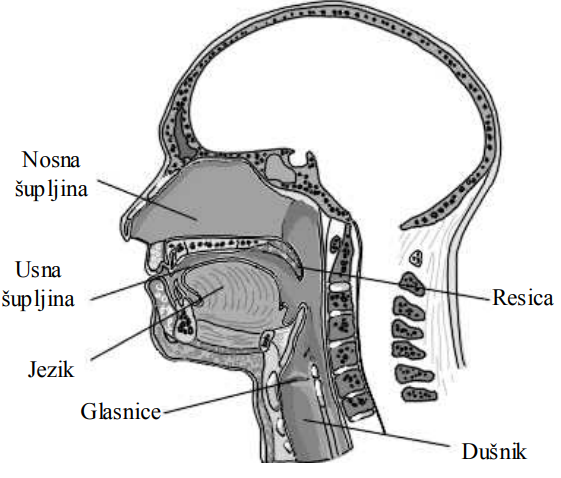
\includegraphics[width=0.6\linewidth]{Chapters/struktura_sustava/generiranje_znacajki/glas.png} 
    \caption{Presjek glave i osnovni dijelovi vokalnog trakta koji sudjeluju u produkciji govornog signala \cite{petrinovic2002}}
    \label{pic:glas}
\end{figure}

Glasnice (engl. glottis) su vrlo značajan organ u procesu formiranja govora. 
Ponašaju se kao mehanički
oscilator koji prelazi u stanje relaksacijskih oscilacija uslijed struje zraka iz pluća koja kroz njih
prolazi. Na frekvenciju njihovog titranja utječu brojni parametri, a među najznačajnijim su
pritisak zraka iz pluća na ulazu u glasnice i napetost samih glasnica.
Takvim periodičkim titranjem, glasnice formiraju periodičku struju zraka, tj. 
kvazi-periodične impulse (engl. glottal pulse) koja zatim prolaze kroz ostatak 
vokalnog trakta što vodi do stvaranja artikuliranih glasova. U slučaju da 
su glasnice potpuno opuštene, neće
doći do oscilacija i struja zraka iz pluća će neometano prolaziti kroz vokalni trakt 
(tada se ne formira kvazi-periodični impuls, nego je rezultat prolaska zraka kroz glasnice
slučajni šum, a rezultat cijelog procesa je stvaranje neartikuliranih glasova). 

S druge strane, vokalni trakt se ponaša kao filtar koji spektralno mijenja karakteristiku
pobudnog signala (engl. vocal tract frequency response). 
Geometrijom vokalnog trakta, koja se mijenja ovisno o položaju 
artikulatora kao što su jezik, usne, čeljust i resica, bit će određen ton (visina i
spektralni sastav) formiranog signala (govora) \cite{petrinovic2002}. 

Jednostavni model koji se koristi u području obrade prirodnog govora je da se on 
može prikazati kao izlaz iz linearnog, vremenski promjenjivog sustava čija se 
svojstva sporo mijenjaju s vremenom. Međutim, ako se promatraju dovoljno kratki
segmenti govornog signala, svaki se segment može učinkovito modelirati kao izlaz
iz linearnog, vremenski invarijantnog sustava pobuđenog bilo
kvazi-periodičnim impulsima bilo slučajnim šumom (engl. random noise signal).
Opisani sustav može se prikazati jednadžbom \ref{eq:govor}

\begin{equation}
    \label{eq:govor}
    X(f) = E(f) \cdot H(f)
\end{equation}

gdje je:
\begin{itemize}
    \item \(X(f)\) odziv sustava (govor),
    \item \(E(f)\) pobuda (kvazi-periodični impuls),
    \item \(H(f)\) prijenosna funkcija vokalnog trakta.
\end{itemize}

U vremenskoj domeni isti sustav može se prikazati jednadžbom \ref{eq:govor_vremenska}.
Množenju u frekvencijskoj domeni istovjetna je konvolucija u vremenskoj (i obratno!).

\begin{equation}
    \label{eq:govor_vremenska}
    x(t) = e(t) \ast h(t)
\end{equation}

Cilj ovakvog modeliranja je pronaći bitne informacije u govornom signalu. Pretpostavka na
kojoj se temelji daljnji rad je da je skoro sva informacija iz govornog signala sadržana
u prijenosnoj funkciji govornog trakta, tj. pobuda (kvazi-periodični impulsi) ostaje
konstantnna tijekom govora (veliko pojednostavljenje, međutim svi modeli na kojima
se temelji ovo područje zasnivaju na ovoj činjenici \cite{multiplier, emotion, sidhu2024mfcc}).
Zbog toga želimo pronaći način za 
razdvajanje tih dvaju elemenata modela. Ako primijenimo logaritamsku funkciju na
sustav opisan u frekvencijskoj domeni proizlazi \ref{eq:logaritam}.

\begin{equation}
    \label{eq:logaritam}
    \begin{aligned}
        \log(X(f)) &= \log(E(f) \cdot H(f)) \\
        \log(X(f)) &= \log(E(f)) + \log(H(f))
    \end{aligned}
\end{equation}

Prikazanim su uspješno razdvojeni elementi modela, tj. vidljiv je rastav na zbrojnike
ako se primijeni logaritamska skala. Na slici \ref{pic:rastav} prikazan je utjecaj
komponenata modela na konačni rezultat, a to je glas (engl. speech). 

\begin{figure}[htb]
    \centering
    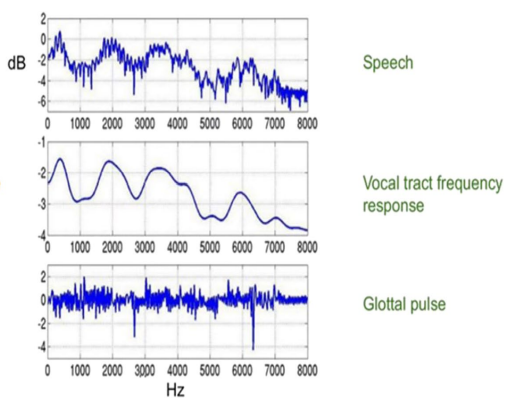
\includegraphics[width=0.6\linewidth]{Chapters/struktura_sustava/generiranje_znacajki/log.png} 
    \caption{Glasovni signal rastavljen na pobudu i odziv vokalnog trakta \cite{sidhu2024mfcc}}
    \label{pic:rastav}
\end{figure}

Jedino što preostaje je pronaći način za što efikasniji opis odziva vokalnog trakta. On će
u konačnici predstavljati zvučne zapise na kojima će model neuronske mreže biti treniran.
U području automatskog prepoznavanja govora te identifikaciji govornika uvelike se koriste
Mel kepstralni vektori.


\subsection{MFCC}
\label{MFCCconstruction}
Mel kepstralni vektori (engl. Mel frequency cepstral coefficients ili MFCC), tj. mjera 
euklidska udaljenosti MFCC vektora jedna je od najčešće korištenih mjera u automatskom 
prepoznavanju govora i govornika \cite{vasilijevic2011perceptual}.





\subsubsection{Window}
\subsubsection{FFT}
\subsubsection{Mel Filterbank}
\subsubsection{DCT}

\subsection{Konstrukcija feature mape}

